\documentclass{article}

\usepackage{fancyhdr} % Required for custom headers
\usepackage{lastpage} % Required to determine the last page for the footer
\usepackage{amsmath}
\usepackage{amsfonts}
\usepackage{graphicx}
\usepackage{listings} 
\usepackage[hidelinks]{hyperref}
% \usepackage{epstopdf} uncomment this line if using MiKTeX

% Margins
\topmargin=-0.45in
\evensidemargin=0in
\oddsidemargin=0in
\textwidth=6.5in
\textheight=9.0in
\headsep=0.25in 

\linespread{1.25} % Line spacing

% Set up the header and footer
\pagestyle{fancy}
\lhead{\authorName} % Top left header
\chead{\classID\ \hwTitle} % Top center header
\rhead{\studentID} % Top right header
\lfoot{} % Bottom left footer
\cfoot{} % Bottom center footer
\rfoot{Page\ \thepage\ of~\pageref{LastPage}} % Bottom right footer
\renewcommand{\headrulewidth}{0.4pt} % Size of the header rule
\renewcommand{\footrulewidth}{0.4pt} % Size of the footer rule

\setlength{\parindent}{0pt} % Removes all indentation from paragraphs

\setcounter{secnumdepth}{0} % Removes default section numbers
\newcounter{problemCounter} % Creates a counter to keep track of the number of problems

\newcommand{\problemName}{}
\newenvironment{problem}[1][Problem \arabic{problemCounter}]{
	\stepcounter{problemCounter} % Increase counter for number of problems
	\renewcommand{\problemName}{#1} % Assign \problemName the name of the problem
	\section{\problemName} % Make a section in the document with the custom problem count
}{}

\newcommand{\subproblemName}{}
	\newenvironment{subproblem}[1]{
	\renewcommand{\subproblemName}{#1} % Assign \subproblemName to the name of the section from the environment argument
	\subsection{\subproblemName} % Make a subsection with the custom name of the subsection
}{}

%----------------------------------------------------------------------------------------
%	MATH OPERATOR
%----------------------------------------------------------------------------------------

\DeclareMathOperator*{\argmin}{arg\,min}
\DeclareMathOperator*{\argmax}{arg\,max}

%----------------------------------------------------------------------------------------
%	NAME AND CLASS SECTION
%----------------------------------------------------------------------------------------

\newcommand{\hwTitle}{Assignment\ \#1} % Assignment title
\newcommand{\dueDate}{Thursday,\ March\ 3,\ 2015} % Due date
\newcommand{\classID}{ENGG\ 5202} % Course/Class
\newcommand{\authorName}{Kai Chen} % Your name
\newcommand{\studentID}{1155070509} % Your student ID

%----------------------------------------------------------------------------------------
%	TITLE PAGE
%----------------------------------------------------------------------------------------

\title{
	\vspace{2in}
	\textmd{\textbf{\classID:\ \hwTitle}}\\
	\normalsize\vspace{0.1in}\small{Due\ on\ \dueDate}
	\vspace{3in}
}

\author{\textbf{\authorName}}
\date{} % Insert date here if you want it to appear below your name

%----------------------------------------------------------------------------------------

\begin{document}
\maketitle
\setcounter{page}{0}
\thispagestyle{empty}
\newpage

%----------------------------------------------------------------------------------------
%	PROBLEM 1
%----------------------------------------------------------------------------------------

% To have just one problem per page, simply put a \clearpage after each problem

\begin{problem}

The likelihood of $\theta_1$
\[
	p(D_1|\theta_1) = p(x_1|\omega_1,\theta_1)p(x_2|\omega_1,\theta_1)
\]
The log-likelihood
\[
	l(\theta_1) = \log p(x_1|\omega_1,\theta_1) = \log p(x_1|\omega_1,\theta_1) + \log p(x_2|\omega_1,\theta_1)
\]
We determine $\theta_1$ by maximizing $l(\theta_1)$
\[
	\hat{\theta_1} = \argmax l(\theta_1)
\]
Let
\[
	\nabla l(\theta_1) = 0
\]
By substituting symbols with numeral values
\begin{eqnarray*}
	l(\theta_1) &=& 2\log\frac{2}{\theta_1} + \log(1-\frac{2}{\theta_1}) + \log(1-\frac{5}{\theta_1}) \\
	\nabla l(\theta_1) &=& - \frac{4}{\theta_1} + \frac{4}{\theta_1(\theta_1-2)} + \frac{10}{\theta_1(\theta_1-5)}	
\end{eqnarray*}
We get 
\[
	\theta_1=8 \quad or \quad \theta_1=2.5
\]
However, \( p(x|\omega_1)=0 \) when \( x>\theta_1 \) according to the densities form, if \( \theta_1=2.5 \), then \( D_1=\{2,5\} \) will not occur. Thus \( \theta_1=8 \).

Similarly, we can calculate \( \theta_2\approx14.2 \)

\end{problem}

%----------------------------------------------------------------------------------------
%	PROBLEM 2
%----------------------------------------------------------------------------------------

\begin{problem}

%-------------------2.1-----------------------

\begin{subproblem}{2.1}

Figure~\ref{fig:p2_1} shows \( p(x|\theta) \) versus \( x \) for \( \theta=1 \).

\begin{figure}[htbp]
\centering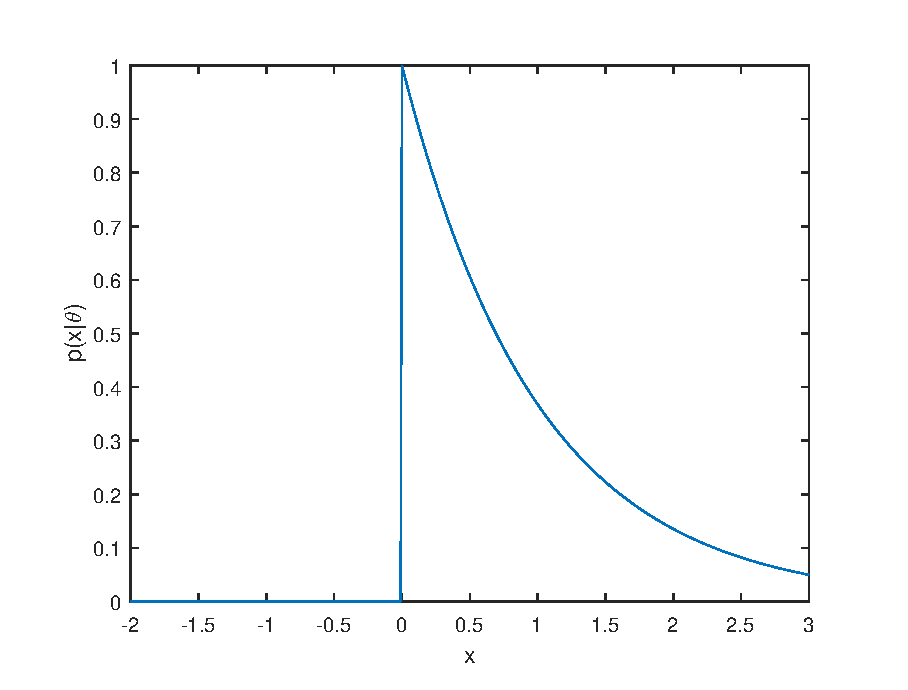
\includegraphics[width=4in]{image/p2_1}
\caption{\( p(x|\theta) \) versus \( x \) for \( \theta=1 \)}\label{fig:p2_1}
\end{figure}

Figure~\ref{fig:p2_2} shows \( p(x|\theta) \) versus \( \theta \) for \( x=2 \).

\begin{figure}[htbp]
\centering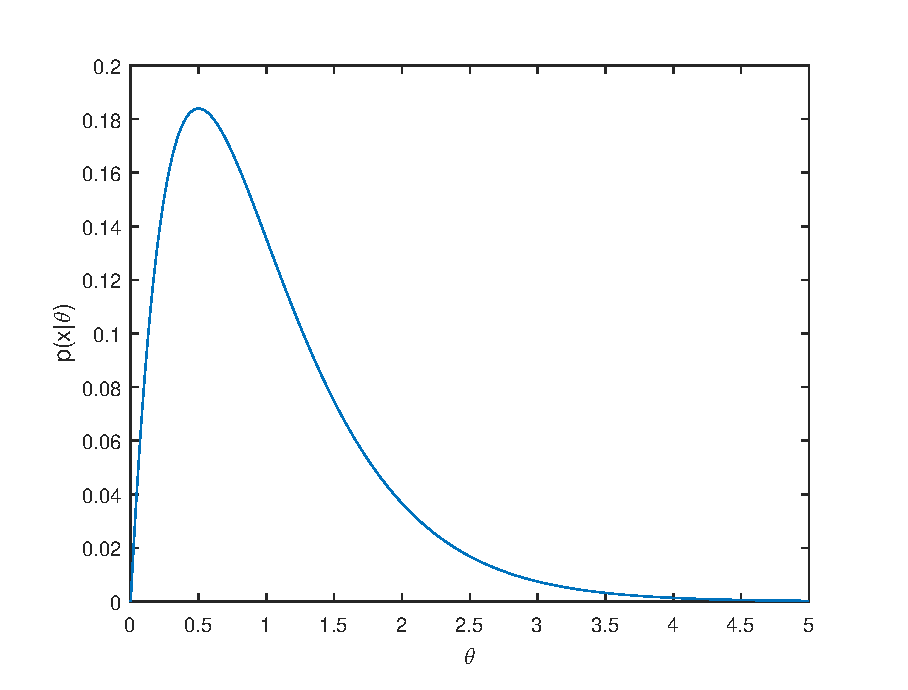
\includegraphics[width=4in]{image/p2_2}
\caption{\( p(x|\theta) \) versus \( \theta \) for \( x=2 \)}\label{fig:p2_2}
\end{figure}

\end{subproblem}

%---------------------2.2---------------------

\begin{subproblem}{2.2}

The log-likelihood

\[
\begin{split}
	l(\theta) &= \log \prod_{k=1}^n p(x_k|\theta) \\
	&= \sum_{k=1}^n \log \theta\mathrm{e}^{-\theta x_k}
\end{split}
\]

The gradient of \( l(\theta) \)

\[
\begin{split}
	\nabla l(\theta) & = \sum_{k=1}^n \frac{(1-\theta x_k)\mathrm{e}^{-\theta x_k}}{\theta\mathrm{e}^{-\theta x_k}} \\
	&= \sum_{k=1}^n \frac{1-\theta x_k}{\theta} \\ 
	&= \frac{n-\theta \sum_{k=1}^n x_k}{\theta}
\end{split}
\]

Let \( \nabla l(\theta) = 0 \), we can calculate

\[
	\hat{\theta} = \frac{n}{\sum_{k=1}^n x_k}
\]

\end{subproblem}

%--------------------2.3----------------------

\begin{subproblem}{2.3}

According to the law of large numbers, when \( n \) is very large, the sample average converges to the expected value.

\[
	\frac{\sum_{k=1}^n x_k}{n} \rightarrow \mathcal{E}(x) = \int_0^{\infty}\theta x\mathrm{e}^{-\theta x}\,\mathrm{d}x = \frac{1}{\theta}
\]

So \( \hat{\theta} \) approach to the true \( \theta \) when n is very large. If the samples are generated from \( p(x|\theta) \) with \( \theta=1 \), the maximum-likelihood estimate \( \hat{\theta} \) for large n is 1.

\end{subproblem}

\end{problem}

%----------------------------------------------------------------------------------------
%	PROBLEM 3
%----------------------------------------------------------------------------------------

\begin{problem}

%--------------------3.1----------------------

\begin{subproblem}{3.1}

\begin{align*}
	p(x_k|\theta^{(t)}) &= \sum_{j=1}^m\sum_{i=1}^l p_j^{(t)}q_i^{(t)}N(x_k;\mu_j^{(t)},{\sigma_i^{(t)}}^2) \\ \\
	p(z_k,y_k,x_k|\theta^{(t)}) &= p_{z_k}q_{y_k}N(x_k;\mu_{z_k}^{(t)},\sigma_{y_k}^{(t)}) \\ \\
	p(z_k,y_k;x_k,\theta^{(t)}) &= \frac{p(z_k,y_k,x_k|\theta^{(t)})}{p(x_k|\theta^{(t)})} \\
	&= \frac{p_{z_k}q_{y_k}N(x_k;\mu_{z_k}^{(t)},\sigma_{y_k}^{(t)})}{\sum_{j=1}^m\sum_{i=1}^l p_j\,q_iN(x_k;\mu_j^{(t)},{\sigma_i^{(t)}}^2)}
\end{align*}

\end{subproblem}

%--------------------3.2----------------------

\begin{subproblem}{3.2}

\[
	l_c(x_1,\dots,x_n,z_1,\dots,z_n,y_1,\dots,y_n;\theta) = \sum_{k=1}^n\log(p_{z_k}q_{y_k}N(x_k;\mu_{z_k}^{(t)},\sigma_{y_k}^{(t)}))
\]
\begin{align*}
	Q(\theta;\theta^{(t)}) &= \mathcal{E}\{l_c(x_1,\dots,x_n,z_1,\dots,z_n,y_1,\dots,y_n;\theta)|x_1,\dots,x_n,\theta^{(t)}\} \\
	&= \sum_{k=1}^n\mathcal{E}\{\log(p_{z_k}q_{y_k}N(x_k;\mu_{z_k}^{(t)},\sigma_{y_k}^{(t)}))|x_k,\theta^{(t)}\} \\
	&= \sum_{k=1}^n\sum_{j=1}^m\sum_{i=1}^l\,P(z_k=j,y_k=i|x_k,\theta^{(t)})\log(p_j\,q_iN(x_k;\mu_j,{\sigma_i^2)})
\end{align*}

\end{subproblem}

%--------------------3.3----------------------

\begin{subproblem}{3.3}

\[
	\mbox{Let}\frac{\partial Q(\theta;\theta^{(t)})}{\partial\mu_j} = \sum_{k=1}^n\sum_{i=1}^l\,P(z_k=j,y_k=i|x_k,\theta^{(t)})\frac{x_k-\mu_j}{\sigma_i^2} = 0
\]
\[
	\mu_j = \frac{\sum_{k=1}^n\sum_{i=1}^l\,P(z_k=j,y_k=i|x_k,\theta^{(t)})\frac{x_k}{\sigma_i^2}}{\sum_{k=1}^n\sum_{i=1}^l\,P(z_k=j,y_k=i|x_k,\theta^{(t)})\frac{1}{\sigma_i^2}}
\]

\end{subproblem}

%--------------------3.4----------------------

\begin{subproblem}{3.4}

The approximation quality is significantly worse when \(l=1\) than \(l>1\). This is because the data is sampled from a true mixture model with 3 mean parameters and 2 variance parameters, while a mixture model with single variance parameter and many mean parameters has weaker ability to fit the data well due to the degree of freedom. Instead, a mixture model which can adjust multiple variance parameters as well as mean parameters can do better.

\end{subproblem}

\end{problem}

%----------------------------------------------------------------------------------------
%	PROBLEM 4
%----------------------------------------------------------------------------------------

\begin{problem}

%--------------------4.1----------------------

\begin{subproblem}{4.1}

One sequence generated by my program: 2 1 1 1 1 2 2 2 3 1

\end{subproblem}

%--------------------4.2----------------------

\begin{subproblem}{4.2}
The most likely sequence of hidden states: 1 2 2 2 2 1 1 1 1 2 \\
The true hidden states: 2 1 2 2 2 2 2 1 1 1\\
Codes have been submitted to Piazza.
\end{subproblem}

\end{problem}

\end{document}
